\documentclass[1p]{elsarticle_modified}
%\bibliographystyle{elsarticle-num}

%\usepackage[colorlinks]{hyperref}
%\usepackage{abbrmath_seonhwa} %\Abb, \Ascr, \Acal ,\Abf, \Afrak
\usepackage{amsfonts}
\usepackage{amssymb}
\usepackage{amsmath}
\usepackage{amsthm}
\usepackage{scalefnt}
\usepackage{amsbsy}
\usepackage{kotex}
\usepackage{caption}
\usepackage{subfig}
\usepackage{color}
\usepackage{graphicx}
\usepackage{xcolor} %% white, black, red, green, blue, cyan, magenta, yellow
\usepackage{float}
\usepackage{setspace}
\usepackage{hyperref}

\usepackage{tikz}
\usetikzlibrary{arrows}

\usepackage{multirow}
\usepackage{array} % fixed length table
\usepackage{hhline}

%%%%%%%%%%%%%%%%%%%%%
\makeatletter
\renewcommand*\env@matrix[1][\arraystretch]{%
	\edef\arraystretch{#1}%
	\hskip -\arraycolsep
	\let\@ifnextchar\new@ifnextchar
	\array{*\c@MaxMatrixCols c}}
\makeatother %https://tex.stackexchange.com/questions/14071/how-can-i-increase-the-line-spacing-in-a-matrix
%%%%%%%%%%%%%%%

\usepackage[normalem]{ulem}

\newcommand{\msout}[1]{\ifmmode\text{\sout{\ensuremath{#1}}}\else\sout{#1}\fi}
%SOURCE: \msout is \stkout macro in https://tex.stackexchange.com/questions/20609/strikeout-in-math-mode

\newcommand{\cancel}[1]{
	\ifmmode
	{\color{red}\msout{#1}}
	\else
	{\color{red}\sout{#1}}
	\fi
}

\newcommand{\add}[1]{
	{\color{blue}\uwave{#1}}
}

\newcommand{\replace}[2]{
	\ifmmode
	{\color{red}\msout{#1}}{\color{blue}\uwave{#2}}
	\else
	{\color{red}\sout{#1}}{\color{blue}\uwave{#2}}
	\fi
}

\newcommand{\Sol}{\mathcal{S}} %segment
\newcommand{\D}{D} %diagram
\newcommand{\A}{\mathcal{A}} %arc


%%%%%%%%%%%%%%%%%%%%%%%%%%%%%5 test

\def\sl{\operatorname{\textup{SL}}(2,\Cbb)}
\def\psl{\operatorname{\textup{PSL}}(2,\Cbb)}
\def\quan{\mkern 1mu \triangleright \mkern 1mu}

\theoremstyle{definition}
\newtheorem{thm}{Theorem}[section]
\newtheorem{prop}[thm]{Proposition}
\newtheorem{lem}[thm]{Lemma}
\newtheorem{ques}[thm]{Question}
\newtheorem{cor}[thm]{Corollary}
\newtheorem{defn}[thm]{Definition}
\newtheorem{exam}[thm]{Example}
\newtheorem{rmk}[thm]{Remark}
\newtheorem{alg}[thm]{Algorithm}

\newcommand{\I}{\sqrt{-1}}
\begin{document}

%\begin{frontmatter}
%
%\title{Boundary parabolic representations of knots up to 8 crossings}
%
%%% Group authors per affiliation:
%\author{Yunhi Cho} 
%\address{Department of Mathematics, University of Seoul, Seoul, Korea}
%\ead{yhcho@uos.ac.kr}
%
%
%\author{Seonhwa Kim} %\fnref{s_kim}}
%\address{Center for Geometry and Physics, Institute for Basic Science, Pohang, 37673, Korea}
%\ead{ryeona17@ibs.re.kr}
%
%\author{Hyuk Kim}
%\address{Department of Mathematical Sciences, Seoul National University, Seoul 08826, Korea}
%\ead{hyukkim@snu.ac.kr}
%
%\author{Seokbeom Yoon}
%\address{Department of Mathematical Sciences, Seoul National University, Seoul, 08826,  Korea}
%\ead{sbyoon15@snu.ac.kr}
%
%\begin{abstract}
%We find all boundary parabolic representation of knots up to 8 crossings.
%
%\end{abstract}
%\begin{keyword}
%    \MSC[2010] 57M25 
%\end{keyword}
%
%\end{frontmatter}

%\linenumbers
%\tableofcontents
%
\newcommand\colored[1]{\textcolor{white}{\rule[-0.35ex]{0.8em}{1.4ex}}\kern-0.8em\color{red} #1}%
%\newcommand\colored[1]{\textcolor{white}{ #1}\kern-2.17ex	\textcolor{white}{ #1}\kern-1.81ex	\textcolor{white}{ #1}\kern-2.15ex\color{red}#1	}

{\Large $\underline{12n_{0648}~(K12n_{0648})}$}

\setlength{\tabcolsep}{10pt}
\renewcommand{\arraystretch}{1.6}
\vspace{1cm}\begin{tabular}{m{100pt}>{\centering\arraybackslash}m{274pt}}
\multirow{5}{120pt}{
	\centering
	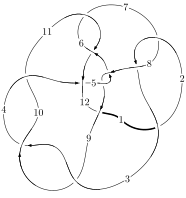
\includegraphics[width=112pt]{../../../GIT/diagram.site/Diagrams/png/2737_12n_0648.png}\\
\ \ \ A knot diagram\footnotemark}&
\allowdisplaybreaks
\textbf{Linearized knot diagam} \\
\cline{2-2}
 &
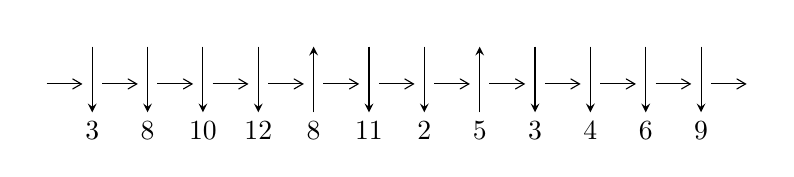
\begin{tikzpicture}[x=20pt, y=17pt]
	% nodes
	\node (C0) at (0, 0) {};
	\node (C1) at (1, 0) {};
	\node (C1U) at (1, +1) {};
	\node (C1D) at (1, -1) {3};

	\node (C2) at (2, 0) {};
	\node (C2U) at (2, +1) {};
	\node (C2D) at (2, -1) {8};

	\node (C3) at (3, 0) {};
	\node (C3U) at (3, +1) {};
	\node (C3D) at (3, -1) {10};

	\node (C4) at (4, 0) {};
	\node (C4U) at (4, +1) {};
	\node (C4D) at (4, -1) {12};

	\node (C5) at (5, 0) {};
	\node (C5U) at (5, +1) {};
	\node (C5D) at (5, -1) {8};

	\node (C6) at (6, 0) {};
	\node (C6U) at (6, +1) {};
	\node (C6D) at (6, -1) {11};

	\node (C7) at (7, 0) {};
	\node (C7U) at (7, +1) {};
	\node (C7D) at (7, -1) {2};

	\node (C8) at (8, 0) {};
	\node (C8U) at (8, +1) {};
	\node (C8D) at (8, -1) {5};

	\node (C9) at (9, 0) {};
	\node (C9U) at (9, +1) {};
	\node (C9D) at (9, -1) {3};

	\node (C10) at (10, 0) {};
	\node (C10U) at (10, +1) {};
	\node (C10D) at (10, -1) {4};

	\node (C11) at (11, 0) {};
	\node (C11U) at (11, +1) {};
	\node (C11D) at (11, -1) {6};

	\node (C12) at (12, 0) {};
	\node (C12U) at (12, +1) {};
	\node (C12D) at (12, -1) {9};
	\node (C13) at (13, 0) {};

	% arrows
	\draw[->,>={angle 60}]
	(C0) edge (C1) (C1) edge (C2) (C2) edge (C3) (C3) edge (C4) (C4) edge (C5) (C5) edge (C6) (C6) edge (C7) (C7) edge (C8) (C8) edge (C9) (C9) edge (C10) (C10) edge (C11) (C11) edge (C12) (C12) edge (C13) ;	\draw[->,>=stealth]
	(C1U) edge (C1D) (C2U) edge (C2D) (C3U) edge (C3D) (C4U) edge (C4D) (C5D) edge (C5U) (C6U) edge (C6D) (C7U) edge (C7D) (C8D) edge (C8U) (C9U) edge (C9D) (C10U) edge (C10D) (C11U) edge (C11D) (C12U) edge (C12D) ;
	\end{tikzpicture} \\
\hhline{~~} \\& 
\textbf{Solving Sequence} \\ \cline{2-2} 
 &
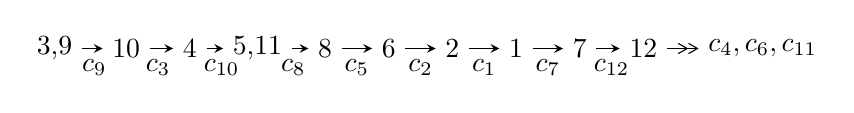
\begin{tikzpicture}[x=23pt, y=7pt]
	% node
	\node (A0) at (-1/8, 0) {3,9};
	\node (A1) at (1, 0) {10};
	\node (A2) at (2, 0) {4};
	\node (A3) at (49/16, 0) {5,11};
	\node (A4) at (33/8, 0) {8};
	\node (A5) at (41/8, 0) {6};
	\node (A6) at (49/8, 0) {2};
	\node (A7) at (57/8, 0) {1};
	\node (A8) at (65/8, 0) {7};
	\node (A9) at (73/8, 0) {12};
	\node (C1) at (1/2, -1) {$c_{9}$};
	\node (C2) at (3/2, -1) {$c_{3}$};
	\node (C3) at (5/2, -1) {$c_{10}$};
	\node (C4) at (29/8, -1) {$c_{8}$};
	\node (C5) at (37/8, -1) {$c_{5}$};
	\node (C6) at (45/8, -1) {$c_{2}$};
	\node (C7) at (53/8, -1) {$c_{1}$};
	\node (C8) at (61/8, -1) {$c_{7}$};
	\node (C9) at (69/8, -1) {$c_{12}$};
	\node (A10) at (11, 0) {$c_{4},c_{6},c_{11}$};

	% edge
	\draw[->,>=stealth]	
	(A0) edge (A1) (A1) edge (A2) (A2) edge (A3) (A3) edge (A4) (A4) edge (A5) (A5) edge (A6) (A6) edge (A7) (A7) edge (A8) (A8) edge (A9) ;
	\draw[->>,>={angle 60}]	
	(A9) edge (A10);
\end{tikzpicture} \\ 

\end{tabular} \\

\footnotetext{
The image of knot diagram is generated by the software ``\textbf{Draw programme}" developed by Andrew Bartholomew(\url{http://www.layer8.co.uk/maths/draw/index.htm\#Running-draw}), where we modified some parts for our purpose(\url{https://github.com/CATsTAILs/LinksPainter}).
}\phantom \\ \newline 
\centering \textbf{Ideals for irreducible components\footnotemark of $X_{\text{par}}$} 
 
\begin{align*}
I^u_{1}&=\langle 
-6.95358\times10^{37} u^{23}-4.07407\times10^{36} u^{22}+\cdots+1.61095\times10^{39} b-9.52256\times10^{39},\\
\phantom{I^u_{1}}&\phantom{= \langle  }-7.06431\times10^{39} u^{23}+8.51893\times10^{38} u^{22}+\cdots+2.30366\times10^{41} a-7.64291\times10^{41},\\
\phantom{I^u_{1}}&\phantom{= \langle  }u^{24}+u^{23}+\cdots+289 u+143\rangle \\
I^u_{2}&=\langle 
- u^{18}- u^{17}+\cdots+b-1,\;-2 u^{16}- u^{15}+\cdots+a-1,\;u^{19}-12 u^{17}+\cdots+4 u-1\rangle \\
\\
\end{align*}
\raggedright * 2 irreducible components of $\dim_{\mathbb{C}}=0$, with total 43 representations.\\
\footnotetext{All coefficients of polynomials are rational numbers. But the coefficients are sometimes approximated in decimal forms when there is not enough margin.}
\newpage
\renewcommand{\arraystretch}{1}
\centering \section*{I. $I^u_{1}= \langle -6.95\times10^{37} u^{23}-4.07\times10^{36} u^{22}+\cdots+1.61\times10^{39} b-9.52\times10^{39},\;-7.06\times10^{39} u^{23}+8.52\times10^{38} u^{22}+\cdots+2.30\times10^{41} a-7.64\times10^{41},\;u^{24}+u^{23}+\cdots+289 u+143 \rangle$}
\flushleft \textbf{(i) Arc colorings}\\
\begin{tabular}{m{7pt} m{180pt} m{7pt} m{180pt} }
\flushright $a_{3}=$&$\begin{pmatrix}0\\u\end{pmatrix}$ \\
\flushright $a_{9}=$&$\begin{pmatrix}1\\0\end{pmatrix}$ \\
\flushright $a_{10}=$&$\begin{pmatrix}1\\u^2\end{pmatrix}$ \\
\flushright $a_{4}=$&$\begin{pmatrix}- u\\- u^3+u\end{pmatrix}$ \\
\flushright $a_{5}=$&$\begin{pmatrix}0.0306656 u^{23}-0.00369799 u^{22}+\cdots+2.32158 u+3.31772\\0.0431644 u^{23}+0.00252898 u^{22}+\cdots+7.19118 u+5.91114\end{pmatrix}$ \\
\flushright $a_{11}=$&$\begin{pmatrix}- u^2+1\\- u^4+2 u^2\end{pmatrix}$ \\
\flushright $a_{8}=$&$\begin{pmatrix}0.0142787 u^{23}-0.00544253 u^{22}+\cdots+2.94433 u+2.42345\\0.0139246 u^{23}-0.0131718 u^{22}+\cdots+1.01894 u+0.464061\end{pmatrix}$ \\
\flushright $a_{6}=$&$\begin{pmatrix}0.0251613 u^{23}-0.000730907 u^{22}+\cdots+1.76692 u+2.55543\\-0.0181599 u^{23}+0.00533470 u^{22}+\cdots-1.56432 u-1.98558\end{pmatrix}$ \\
\flushright $a_{2}=$&$\begin{pmatrix}-0.0497304 u^{23}+0.00323432 u^{22}+\cdots-6.95114 u-7.14443\\-0.0419268 u^{23}-0.00473941 u^{22}+\cdots-4.93122 u-6.22408\end{pmatrix}$ \\
\flushright $a_{1}=$&$\begin{pmatrix}-0.0497304 u^{23}+0.00323432 u^{22}+\cdots-6.95114 u-7.14443\\0.0148906 u^{23}-0.00607853 u^{22}+\cdots+3.26414 u+1.34988\end{pmatrix}$ \\
\flushright $a_{7}=$&$\begin{pmatrix}-0.0265932 u^{23}-0.00297561 u^{22}+\cdots-2.70453 u-3.73203\\0.00559528 u^{23}-0.00695287 u^{22}+\cdots+0.504854 u+0.119250\end{pmatrix}$ \\
\flushright $a_{12}=$&$\begin{pmatrix}-0.0348398 u^{23}-0.00284421 u^{22}+\cdots-3.68700 u-5.79455\\0.0148906 u^{23}-0.00607853 u^{22}+\cdots+3.26414 u+1.34988\end{pmatrix}$\\&\end{tabular}
\flushleft \textbf{(ii) Obstruction class $= -1$}\\~\\
\flushleft \textbf{(iii) Cusp Shapes $= -0.0449908 u^{23}+0.00298260 u^{22}+\cdots-19.5117 u-16.1952$}\\~\\
\newpage\renewcommand{\arraystretch}{1}
\flushleft \textbf{(iv) u-Polynomials at the component}\newline \\
\begin{tabular}{m{50pt}|m{274pt}}
Crossings & \hspace{64pt}u-Polynomials at each crossing \\
\hline $$\begin{aligned}c_{1}\end{aligned}$$&$\begin{aligned}
&u^{24}+60 u^{23}+\cdots+3708160 u+295936
\end{aligned}$\\
\hline $$\begin{aligned}c_{2},c_{7}\end{aligned}$$&$\begin{aligned}
&u^{24}-10 u^{23}+\cdots+16 u+544
\end{aligned}$\\
\hline $$\begin{aligned}c_{3},c_{9},c_{10}\end{aligned}$$&$\begin{aligned}
&u^{24}- u^{23}+\cdots-289 u+143
\end{aligned}$\\
\hline $$\begin{aligned}c_{4}\end{aligned}$$&$\begin{aligned}
&u^{24}+3 u^{23}+\cdots-327 u-41
\end{aligned}$\\
\hline $$\begin{aligned}c_{5},c_{8}\end{aligned}$$&$\begin{aligned}
&u^{24}+2 u^{23}+\cdots+13 u-1
\end{aligned}$\\
\hline $$\begin{aligned}c_{6},c_{11}\end{aligned}$$&$\begin{aligned}
&u^{24}- u^{23}+\cdots-288 u-69
\end{aligned}$\\
\hline $$\begin{aligned}c_{12}\end{aligned}$$&$\begin{aligned}
&u^{24}-36 u^{22}+\cdots-47638 u-14543
\end{aligned}$\\
\hline
\end{tabular}\\~\\
\newpage\renewcommand{\arraystretch}{1}
\flushleft \textbf{(v) Riley Polynomials at the component}\newline \\
\begin{tabular}{m{50pt}|m{274pt}}
Crossings & \hspace{64pt}Riley Polynomials at each crossing \\
\hline $$\begin{aligned}c_{1}\end{aligned}$$&$\begin{aligned}
&y^{24}-296 y^{23}+\cdots-4939910283264 y+87578116096
\end{aligned}$\\
\hline $$\begin{aligned}c_{2},c_{7}\end{aligned}$$&$\begin{aligned}
&y^{24}-60 y^{23}+\cdots-3708160 y+295936
\end{aligned}$\\
\hline $$\begin{aligned}c_{3},c_{9},c_{10}\end{aligned}$$&$\begin{aligned}
&y^{24}-45 y^{23}+\cdots-70079 y+20449
\end{aligned}$\\
\hline $$\begin{aligned}c_{4}\end{aligned}$$&$\begin{aligned}
&y^{24}-11 y^{23}+\cdots-33785 y+1681
\end{aligned}$\\
\hline $$\begin{aligned}c_{5},c_{8}\end{aligned}$$&$\begin{aligned}
&y^{24}+26 y^{23}+\cdots-575 y+1
\end{aligned}$\\
\hline $$\begin{aligned}c_{6},c_{11}\end{aligned}$$&$\begin{aligned}
&y^{24}-9 y^{23}+\cdots-35058 y+4761
\end{aligned}$\\
\hline $$\begin{aligned}c_{12}\end{aligned}$$&$\begin{aligned}
&y^{24}-72 y^{23}+\cdots-2969653580 y+211498849
\end{aligned}$\\
\hline
\end{tabular}\\~\\
\newpage\flushleft \textbf{(vi) Complex Volumes and Cusp Shapes}
$$\begin{array}{c|c|c}  
\text{Solutions to }I^u_{1}& \I (\text{vol} + \sqrt{-1}CS) & \text{Cusp shape}\\
 \hline 
\begin{aligned}
u &= -0.998180 + 0.182421 I \\
a &= -0.371865 + 0.963824 I \\
b &= -0.46248 + 1.36040 I\end{aligned}
 & -2.89773 - 4.47411 I & -11.26620 + 4.32225 I \\ \hline\begin{aligned}
u &= -0.998180 - 0.182421 I \\
a &= -0.371865 - 0.963824 I \\
b &= -0.46248 - 1.36040 I\end{aligned}
 & -2.89773 + 4.47411 I & -11.26620 - 4.32225 I \\ \hline\begin{aligned}
u &= -1.08785\phantom{ +0.000000I} \\
a &= \phantom{-}0.370138\phantom{ +0.000000I} \\
b &= \phantom{-}0.466022\phantom{ +0.000000I}\end{aligned}
 & -5.81657\phantom{ +0.000000I} & -15.7030\phantom{ +0.000000I} \\ \hline\begin{aligned}
u &= -0.908883 + 0.696346 I \\
a &= \phantom{-}0.819047 - 0.748643 I \\
b &= -1.50457 - 0.48587 I\end{aligned}
 & \phantom{-}2.29616 + 2.53148 I & -13.0553 - 13.0894 I \\ \hline\begin{aligned}
u &= -0.908883 - 0.696346 I \\
a &= \phantom{-}0.819047 + 0.748643 I \\
b &= -1.50457 + 0.48587 I\end{aligned}
 & \phantom{-}2.29616 - 2.53148 I & -13.0553 + 13.0894 I \\ \hline\begin{aligned}
u &= -0.369638 + 0.655856 I \\
a &= \phantom{-}0.163913 + 0.088570 I \\
b &= -0.483150 + 1.254690 I\end{aligned}
 & -1.35028 - 2.85129 I & -8.82275 - 0.17568 I \\ \hline\begin{aligned}
u &= -0.369638 - 0.655856 I \\
a &= \phantom{-}0.163913 - 0.088570 I \\
b &= -0.483150 - 1.254690 I\end{aligned}
 & -1.35028 + 2.85129 I & -8.82275 + 0.17568 I \\ \hline\begin{aligned}
u &= \phantom{-}0.351833 + 0.653611 I \\
a &= -1.42495 - 0.28417 I \\
b &= \phantom{-}0.440762 - 1.267520 I\end{aligned}
 & -3.72902 - 2.23669 I & -11.06844 + 3.08943 I \\ \hline\begin{aligned}
u &= \phantom{-}0.351833 - 0.653611 I \\
a &= -1.42495 + 0.28417 I \\
b &= \phantom{-}0.440762 + 1.267520 I\end{aligned}
 & -3.72902 + 2.23669 I & -11.06844 - 3.08943 I \\ \hline\begin{aligned}
u &= \phantom{-}1.312160 + 0.113933 I \\
a &= -0.648596 + 1.219050 I \\
b &= \phantom{-}0.265262 + 0.114333 I\end{aligned}
 & -2.00982 - 3.68666 I & -7.35603 + 5.27682 I\\
 \hline 
 \end{array}$$\newpage$$\begin{array}{c|c|c}  
\text{Solutions to }I^u_{1}& \I (\text{vol} + \sqrt{-1}CS) & \text{Cusp shape}\\
 \hline 
\begin{aligned}
u &= \phantom{-}1.312160 - 0.113933 I \\
a &= -0.648596 - 1.219050 I \\
b &= \phantom{-}0.265262 - 0.114333 I\end{aligned}
 & -2.00982 + 3.68666 I & -7.35603 - 5.27682 I \\ \hline\begin{aligned}
u &= -1.42954 + 0.07398 I \\
a &= -0.35156 - 1.37276 I \\
b &= \phantom{-}0.443663 - 1.115380 I\end{aligned}
 & -9.16253 - 3.52152 I & -17.4723 + 4.9311 I \\ \hline\begin{aligned}
u &= -1.42954 - 0.07398 I \\
a &= -0.35156 + 1.37276 I \\
b &= \phantom{-}0.443663 + 1.115380 I\end{aligned}
 & -9.16253 + 3.52152 I & -17.4723 - 4.9311 I \\ \hline\begin{aligned}
u &= -0.172334 + 0.521929 I \\
a &= \phantom{-}0.57148 - 1.66997 I \\
b &= -0.572916 + 0.049432 I\end{aligned}
 & \phantom{-}2.32011 + 1.43982 I & -3.19830 - 4.08238 I \\ \hline\begin{aligned}
u &= -0.172334 - 0.521929 I \\
a &= \phantom{-}0.57148 + 1.66997 I \\
b &= -0.572916 - 0.049432 I\end{aligned}
 & \phantom{-}2.32011 - 1.43982 I & -3.19830 + 4.08238 I \\ \hline\begin{aligned}
u &= \phantom{-}0.406773\phantom{ +0.000000I} \\
a &= -0.663948\phantom{ +0.000000I} \\
b &= \phantom{-}0.198801\phantom{ +0.000000I}\end{aligned}
 & -0.603529\phantom{ +0.000000I} & -16.4560\phantom{ +0.000000I} \\ \hline\begin{aligned}
u &= \phantom{-}1.77917\phantom{ +0.000000I} \\
a &= \phantom{-}0.251024\phantom{ +0.000000I} \\
b &= -0.0435926\phantom{ +0.000000I}\end{aligned}
 & -16.2026\phantom{ +0.000000I} & -29.6210\phantom{ +0.000000I} \\ \hline\begin{aligned}
u &= -2.04114 + 0.56230 I \\
a &= -0.502493 + 0.953370 I \\
b &= \phantom{-}1.10365 + 1.70631 I\end{aligned}
 & \phantom{-}14.2564 + 11.7505 I & -11.51618 - 4.21495 I \\ \hline\begin{aligned}
u &= -2.04114 - 0.56230 I \\
a &= -0.502493 - 0.953370 I \\
b &= \phantom{-}1.10365 - 1.70631 I\end{aligned}
 & \phantom{-}14.2564 - 11.7505 I & -11.51618 + 4.21495 I \\ \hline\begin{aligned}
u &= \phantom{-}2.37547 + 0.30331 I \\
a &= \phantom{-}0.174548 + 1.000270 I \\
b &= -0.11023 + 2.21127 I\end{aligned}
 & \phantom{-}14.5489 - 0.5683 I & -8.00000 + 0. I\phantom{ +0.000000I}\\
 \hline 
 \end{array}$$\newpage$$\begin{array}{c|c|c}  
\text{Solutions to }I^u_{1}& \I (\text{vol} + \sqrt{-1}CS) & \text{Cusp shape}\\
 \hline 
\begin{aligned}
u &= \phantom{-}2.37547 - 0.30331 I \\
a &= \phantom{-}0.174548 - 1.000270 I \\
b &= -0.11023 - 2.21127 I\end{aligned}
 & \phantom{-}14.5489 + 0.5683 I & -8.00000 + 0. I\phantom{ +0.000000I} \\ \hline\begin{aligned}
u &= \phantom{-}2.14046 + 1.17450 I \\
a &= -0.469141 - 0.647096 I \\
b &= \phantom{-}0.27079 - 2.64157 I\end{aligned}
 & -13.27670 - 2.35671 I & \phantom{-0.000000 } 0 \\ \hline\begin{aligned}
u &= \phantom{-}2.14046 - 1.17450 I \\
a &= -0.469141 + 0.647096 I \\
b &= \phantom{-}0.27079 + 2.64157 I\end{aligned}
 & -13.27670 + 2.35671 I & \phantom{-0.000000 } 0 \\ \hline\begin{aligned}
u &= -2.61851\phantom{ +0.000000I} \\
a &= \phantom{-}0.128998\phantom{ +0.000000I} \\
b &= \phantom{-}2.59719\phantom{ +0.000000I}\end{aligned}
 & \phantom{-}18.9868\phantom{ +0.000000I} & -8.00000\phantom{ +0.000000I}\\
 \hline 
 \end{array}$$\newpage\newpage\renewcommand{\arraystretch}{1}
\centering \section*{II. $I^u_{2}= \langle - u^{18}- u^{17}+\cdots+b-1,\;-2 u^{16}- u^{15}+\cdots+a-1,\;u^{19}-12 u^{17}+\cdots+4 u-1 \rangle$}
\flushleft \textbf{(i) Arc colorings}\\
\begin{tabular}{m{7pt} m{180pt} m{7pt} m{180pt} }
\flushright $a_{3}=$&$\begin{pmatrix}0\\u\end{pmatrix}$ \\
\flushright $a_{9}=$&$\begin{pmatrix}1\\0\end{pmatrix}$ \\
\flushright $a_{10}=$&$\begin{pmatrix}1\\u^2\end{pmatrix}$ \\
\flushright $a_{4}=$&$\begin{pmatrix}- u\\- u^3+u\end{pmatrix}$ \\
\flushright $a_{5}=$&$\begin{pmatrix}2 u^{16}+u^{15}+\cdots+6 u+1\\u^{18}+u^{17}+\cdots- u+1\end{pmatrix}$ \\
\flushright $a_{11}=$&$\begin{pmatrix}- u^2+1\\- u^4+2 u^2\end{pmatrix}$ \\
\flushright $a_{8}=$&$\begin{pmatrix}- u^{18}- u^{17}+\cdots+17 u^3-7 u^2\\u^{17}+u^{16}+\cdots+u-1\end{pmatrix}$ \\
\flushright $a_{6}=$&$\begin{pmatrix}u^{17}+2 u^{16}+\cdots-10 u^2+2 u\\u^{16}-10 u^{14}+\cdots+u-1\end{pmatrix}$ \\
\flushright $a_{2}=$&$\begin{pmatrix}u^{18}-12 u^{16}+\cdots-8 u+2\\u^{18}+2 u^{17}+\cdots-7 u+2\end{pmatrix}$ \\
\flushright $a_{1}=$&$\begin{pmatrix}u^{18}-12 u^{16}+\cdots-8 u+2\\u^{18}+2 u^{17}+\cdots-8 u+2\end{pmatrix}$ \\
\flushright $a_{7}=$&$\begin{pmatrix}- u^{18}+12 u^{16}+\cdots+5 u-1\\u^{18}+u^{17}+\cdots+2 u^2-2 u\end{pmatrix}$ \\
\flushright $a_{12}=$&$\begin{pmatrix}2 u^{18}+2 u^{17}+\cdots-16 u+4\\u^{18}+2 u^{17}+\cdots-8 u+2\end{pmatrix}$\\&\end{tabular}
\flushleft \textbf{(ii) Obstruction class $= 1$}\\~\\
\flushleft \textbf{(iii) Cusp Shapes $= - u^{18}-7 u^{17}+4 u^{16}+70 u^{15}+15 u^{14}-288 u^{13}-116 u^{12}+648 u^{11}+286 u^{10}-880 u^9-387 u^8+725 u^7+321 u^6-320 u^5-125 u^4+53 u^3-15 u^2-11 u-7$}\\~\\
\newpage\renewcommand{\arraystretch}{1}
\flushleft \textbf{(iv) u-Polynomials at the component}\newline \\
\begin{tabular}{m{50pt}|m{274pt}}
Crossings & \hspace{64pt}u-Polynomials at each crossing \\
\hline $$\begin{aligned}c_{1}\end{aligned}$$&$\begin{aligned}
&u^{19}-16 u^{18}+\cdots+9 u-1
\end{aligned}$\\
\hline $$\begin{aligned}c_{2}\end{aligned}$$&$\begin{aligned}
&u^{19}-8 u^{17}+\cdots+u+1
\end{aligned}$\\
\hline $$\begin{aligned}c_{3}\end{aligned}$$&$\begin{aligned}
&u^{19}-12 u^{17}+\cdots+4 u+1
\end{aligned}$\\
\hline $$\begin{aligned}c_{4}\end{aligned}$$&$\begin{aligned}
&u^{19}-2 u^{18}+\cdots+5 u^2+1
\end{aligned}$\\
\hline $$\begin{aligned}c_{5}\end{aligned}$$&$\begin{aligned}
&u^{19}+3 u^{18}+\cdots-6 u^2-1
\end{aligned}$\\
\hline $$\begin{aligned}c_{6}\end{aligned}$$&$\begin{aligned}
&u^{19}+2 u^{17}+\cdots- u-1
\end{aligned}$\\
\hline $$\begin{aligned}c_{7}\end{aligned}$$&$\begin{aligned}
&u^{19}-8 u^{17}+\cdots+u-1
\end{aligned}$\\
\hline $$\begin{aligned}c_{8}\end{aligned}$$&$\begin{aligned}
&u^{19}-3 u^{18}+\cdots+6 u^2+1
\end{aligned}$\\
\hline $$\begin{aligned}c_{9},c_{10}\end{aligned}$$&$\begin{aligned}
&u^{19}-12 u^{17}+\cdots+4 u-1
\end{aligned}$\\
\hline $$\begin{aligned}c_{11}\end{aligned}$$&$\begin{aligned}
&u^{19}+2 u^{17}+\cdots- u+1
\end{aligned}$\\
\hline $$\begin{aligned}c_{12}\end{aligned}$$&$\begin{aligned}
&u^{19}- u^{18}+\cdots-39 u-169
\end{aligned}$\\
\hline
\end{tabular}\\~\\
\newpage\renewcommand{\arraystretch}{1}
\flushleft \textbf{(v) Riley Polynomials at the component}\newline \\
\begin{tabular}{m{50pt}|m{274pt}}
Crossings & \hspace{64pt}Riley Polynomials at each crossing \\
\hline $$\begin{aligned}c_{1}\end{aligned}$$&$\begin{aligned}
&y^{19}-32 y^{18}+\cdots-19 y-1
\end{aligned}$\\
\hline $$\begin{aligned}c_{2},c_{7}\end{aligned}$$&$\begin{aligned}
&y^{19}-16 y^{18}+\cdots+9 y-1
\end{aligned}$\\
\hline $$\begin{aligned}c_{3},c_{9},c_{10}\end{aligned}$$&$\begin{aligned}
&y^{19}-24 y^{18}+\cdots-4 y^2-1
\end{aligned}$\\
\hline $$\begin{aligned}c_{4}\end{aligned}$$&$\begin{aligned}
&y^{19}+6 y^{18}+\cdots-10 y-1
\end{aligned}$\\
\hline $$\begin{aligned}c_{5},c_{8}\end{aligned}$$&$\begin{aligned}
&y^{19}+7 y^{18}+\cdots-12 y-1
\end{aligned}$\\
\hline $$\begin{aligned}c_{6},c_{11}\end{aligned}$$&$\begin{aligned}
&y^{19}+4 y^{18}+\cdots-13 y-1
\end{aligned}$\\
\hline $$\begin{aligned}c_{12}\end{aligned}$$&$\begin{aligned}
&y^{19}-7 y^{18}+\cdots-20111 y-28561
\end{aligned}$\\
\hline
\end{tabular}\\~\\
\newpage\flushleft \textbf{(vi) Complex Volumes and Cusp Shapes}
$$\begin{array}{c|c|c}  
\text{Solutions to }I^u_{2}& \I (\text{vol} + \sqrt{-1}CS) & \text{Cusp shape}\\
 \hline 
\begin{aligned}
u &= \phantom{-}0.980950 + 0.604076 I \\
a &= -0.798772 - 0.755373 I \\
b &= \phantom{-}1.49647 - 0.52355 I\end{aligned}
 & \phantom{-}2.48141 - 2.27470 I & \phantom{-}1.66056 - 6.57716 I \\ \hline\begin{aligned}
u &= \phantom{-}0.980950 - 0.604076 I \\
a &= -0.798772 + 0.755373 I \\
b &= \phantom{-}1.49647 + 0.52355 I\end{aligned}
 & \phantom{-}2.48141 + 2.27470 I & \phantom{-}1.66056 + 6.57716 I \\ \hline\begin{aligned}
u &= -0.737628 + 0.359811 I \\
a &= \phantom{-}0.067452 - 0.920420 I \\
b &= -0.762089 + 0.832433 I\end{aligned}
 & -5.41374 - 1.59276 I & -15.0492 + 2.8168 I \\ \hline\begin{aligned}
u &= -0.737628 - 0.359811 I \\
a &= \phantom{-}0.067452 + 0.920420 I \\
b &= -0.762089 - 0.832433 I\end{aligned}
 & -5.41374 + 1.59276 I & -15.0492 - 2.8168 I \\ \hline\begin{aligned}
u &= -1.179440 + 0.170240 I \\
a &= \phantom{-}0.90264 - 1.49402 I \\
b &= -0.490604 - 1.115980 I\end{aligned}
 & -7.08654 + 3.52788 I & -12.56931 - 3.15212 I \\ \hline\begin{aligned}
u &= -1.179440 - 0.170240 I \\
a &= \phantom{-}0.90264 + 1.49402 I \\
b &= -0.490604 + 1.115980 I\end{aligned}
 & -7.08654 - 3.52788 I & -12.56931 + 3.15212 I \\ \hline\begin{aligned}
u &= \phantom{-}1.277010 + 0.114842 I \\
a &= -0.193294 - 0.314119 I \\
b &= \phantom{-}0.305041 - 1.145700 I\end{aligned}
 & -4.51476 - 5.17759 I & -14.4043 + 6.7554 I \\ \hline\begin{aligned}
u &= \phantom{-}1.277010 - 0.114842 I \\
a &= -0.193294 + 0.314119 I \\
b &= \phantom{-}0.305041 + 1.145700 I\end{aligned}
 & -4.51476 + 5.17759 I & -14.4043 - 6.7554 I \\ \hline\begin{aligned}
u &= \phantom{-}1.340980 + 0.147089 I \\
a &= -0.55132 + 2.05499 I \\
b &= \phantom{-}0.135134 + 0.767547 I\end{aligned}
 & -2.81013 - 3.35015 I & -16.3799 + 1.5970 I \\ \hline\begin{aligned}
u &= \phantom{-}1.340980 - 0.147089 I \\
a &= -0.55132 - 2.05499 I \\
b &= \phantom{-}0.135134 - 0.767547 I\end{aligned}
 & -2.81013 + 3.35015 I & -16.3799 - 1.5970 I\\
 \hline 
 \end{array}$$\newpage$$\begin{array}{c|c|c}  
\text{Solutions to }I^u_{2}& \I (\text{vol} + \sqrt{-1}CS) & \text{Cusp shape}\\
 \hline 
\begin{aligned}
u &= -1.42878 + 0.22236 I \\
a &= \phantom{-}0.635513 + 0.360503 I \\
b &= -0.044798 + 0.642597 I\end{aligned}
 & -3.93872 + 0.69346 I & -13.16284 + 0.10930 I \\ \hline\begin{aligned}
u &= -1.42878 - 0.22236 I \\
a &= \phantom{-}0.635513 - 0.360503 I \\
b &= -0.044798 - 0.642597 I\end{aligned}
 & -3.93872 - 0.69346 I & -13.16284 - 0.10930 I \\ \hline\begin{aligned}
u &= \phantom{-}0.353961 + 0.248880 I \\
a &= \phantom{-}0.60428 + 1.70616 I \\
b &= \phantom{-}0.444558 + 1.167630 I\end{aligned}
 & -1.30454 + 3.85459 I & -7.72386 - 6.55740 I \\ \hline\begin{aligned}
u &= \phantom{-}0.353961 - 0.248880 I \\
a &= \phantom{-}0.60428 - 1.70616 I \\
b &= \phantom{-}0.444558 - 1.167630 I\end{aligned}
 & -1.30454 - 3.85459 I & -7.72386 + 6.55740 I \\ \hline\begin{aligned}
u &= \phantom{-}0.112509 + 0.356697 I \\
a &= \phantom{-}3.67512 - 2.27930 I \\
b &= \phantom{-}0.086415 - 0.687232 I\end{aligned}
 & \phantom{-}1.35323 + 1.56259 I & -12.20805 - 3.14313 I \\ \hline\begin{aligned}
u &= \phantom{-}0.112509 - 0.356697 I \\
a &= \phantom{-}3.67512 + 2.27930 I \\
b &= \phantom{-}0.086415 + 0.687232 I\end{aligned}
 & \phantom{-}1.35323 - 1.56259 I & -12.20805 + 3.14313 I \\ \hline\begin{aligned}
u &= -1.62694 + 0.05058 I \\
a &= -0.334359 - 0.989140 I \\
b &= \phantom{-}0.609573 - 1.022040 I\end{aligned}
 & -8.63988 - 2.65005 I & -12.70208 - 1.23601 I \\ \hline\begin{aligned}
u &= -1.62694 - 0.05058 I \\
a &= -0.334359 + 0.989140 I \\
b &= \phantom{-}0.609573 + 1.022040 I\end{aligned}
 & -8.63988 + 2.65005 I & -12.70208 + 1.23601 I \\ \hline\begin{aligned}
u &= \phantom{-}1.81475\phantom{ +0.000000I} \\
a &= -0.0145195\phantom{ +0.000000I} \\
b &= -0.559404\phantom{ +0.000000I}\end{aligned}
 & -15.9196\phantom{ +0.000000I} & -0.921900\phantom{ +0.000000I}\\
 \hline 
 \end{array}$$\newpage
\newpage\renewcommand{\arraystretch}{1}
\centering \section*{ III. u-Polynomials}
\begin{tabular}{m{50pt}|m{274pt}}
Crossings & \hspace{64pt}u-Polynomials at each crossing \\
\hline $$\begin{aligned}c_{1}\end{aligned}$$&$\begin{aligned}
&(u^{19}-16 u^{18}+\cdots+9 u-1)(u^{24}+60 u^{23}+\cdots+3708160 u+295936)
\end{aligned}$\\
\hline $$\begin{aligned}c_{2}\end{aligned}$$&$\begin{aligned}
&(u^{19}-8 u^{17}+\cdots+u+1)(u^{24}-10 u^{23}+\cdots+16 u+544)
\end{aligned}$\\
\hline $$\begin{aligned}c_{3}\end{aligned}$$&$\begin{aligned}
&(u^{19}-12 u^{17}+\cdots+4 u+1)(u^{24}- u^{23}+\cdots-289 u+143)
\end{aligned}$\\
\hline $$\begin{aligned}c_{4}\end{aligned}$$&$\begin{aligned}
&(u^{19}-2 u^{18}+\cdots+5 u^2+1)(u^{24}+3 u^{23}+\cdots-327 u-41)
\end{aligned}$\\
\hline $$\begin{aligned}c_{5}\end{aligned}$$&$\begin{aligned}
&(u^{19}+3 u^{18}+\cdots-6 u^2-1)(u^{24}+2 u^{23}+\cdots+13 u-1)
\end{aligned}$\\
\hline $$\begin{aligned}c_{6}\end{aligned}$$&$\begin{aligned}
&(u^{19}+2 u^{17}+\cdots- u-1)(u^{24}- u^{23}+\cdots-288 u-69)
\end{aligned}$\\
\hline $$\begin{aligned}c_{7}\end{aligned}$$&$\begin{aligned}
&(u^{19}-8 u^{17}+\cdots+u-1)(u^{24}-10 u^{23}+\cdots+16 u+544)
\end{aligned}$\\
\hline $$\begin{aligned}c_{8}\end{aligned}$$&$\begin{aligned}
&(u^{19}-3 u^{18}+\cdots+6 u^2+1)(u^{24}+2 u^{23}+\cdots+13 u-1)
\end{aligned}$\\
\hline $$\begin{aligned}c_{9},c_{10}\end{aligned}$$&$\begin{aligned}
&(u^{19}-12 u^{17}+\cdots+4 u-1)(u^{24}- u^{23}+\cdots-289 u+143)
\end{aligned}$\\
\hline $$\begin{aligned}c_{11}\end{aligned}$$&$\begin{aligned}
&(u^{19}+2 u^{17}+\cdots- u+1)(u^{24}- u^{23}+\cdots-288 u-69)
\end{aligned}$\\
\hline $$\begin{aligned}c_{12}\end{aligned}$$&$\begin{aligned}
&(u^{19}- u^{18}+\cdots-39 u-169)(u^{24}-36 u^{22}+\cdots-47638 u-14543)
\end{aligned}$\\
\hline
\end{tabular}\newpage\renewcommand{\arraystretch}{1}
\centering \section*{ IV. Riley Polynomials}
\begin{tabular}{m{50pt}|m{274pt}}
Crossings & \hspace{64pt}Riley Polynomials at each crossing \\
\hline $$\begin{aligned}c_{1}\end{aligned}$$&$\begin{aligned}
&(y^{19}-32 y^{18}+\cdots-19 y-1)\\
&\cdot(y^{24}-296 y^{23}+\cdots-4939910283264 y+87578116096)
\end{aligned}$\\
\hline $$\begin{aligned}c_{2},c_{7}\end{aligned}$$&$\begin{aligned}
&(y^{19}-16 y^{18}+\cdots+9 y-1)(y^{24}-60 y^{23}+\cdots-3708160 y+295936)
\end{aligned}$\\
\hline $$\begin{aligned}c_{3},c_{9},c_{10}\end{aligned}$$&$\begin{aligned}
&(y^{19}-24 y^{18}+\cdots-4 y^2-1)(y^{24}-45 y^{23}+\cdots-70079 y+20449)
\end{aligned}$\\
\hline $$\begin{aligned}c_{4}\end{aligned}$$&$\begin{aligned}
&(y^{19}+6 y^{18}+\cdots-10 y-1)(y^{24}-11 y^{23}+\cdots-33785 y+1681)
\end{aligned}$\\
\hline $$\begin{aligned}c_{5},c_{8}\end{aligned}$$&$\begin{aligned}
&(y^{19}+7 y^{18}+\cdots-12 y-1)(y^{24}+26 y^{23}+\cdots-575 y+1)
\end{aligned}$\\
\hline $$\begin{aligned}c_{6},c_{11}\end{aligned}$$&$\begin{aligned}
&(y^{19}+4 y^{18}+\cdots-13 y-1)(y^{24}-9 y^{23}+\cdots-35058 y+4761)
\end{aligned}$\\
\hline $$\begin{aligned}c_{12}\end{aligned}$$&$\begin{aligned}
&(y^{19}-7 y^{18}+\cdots-20111 y-28561)\\
&\cdot(y^{24}-72 y^{23}+\cdots-2969653580 y+211498849)
\end{aligned}$\\
\hline
\end{tabular}
\vskip 2pc
\end{document}